% Generated by code/visibility/WritePaper.py from inventory-visibility-v1.
\clearpage
\begin{center}
\begin{minipage}{\linewidth}\centering
\captionsetup{type=figure,hypcap=false}
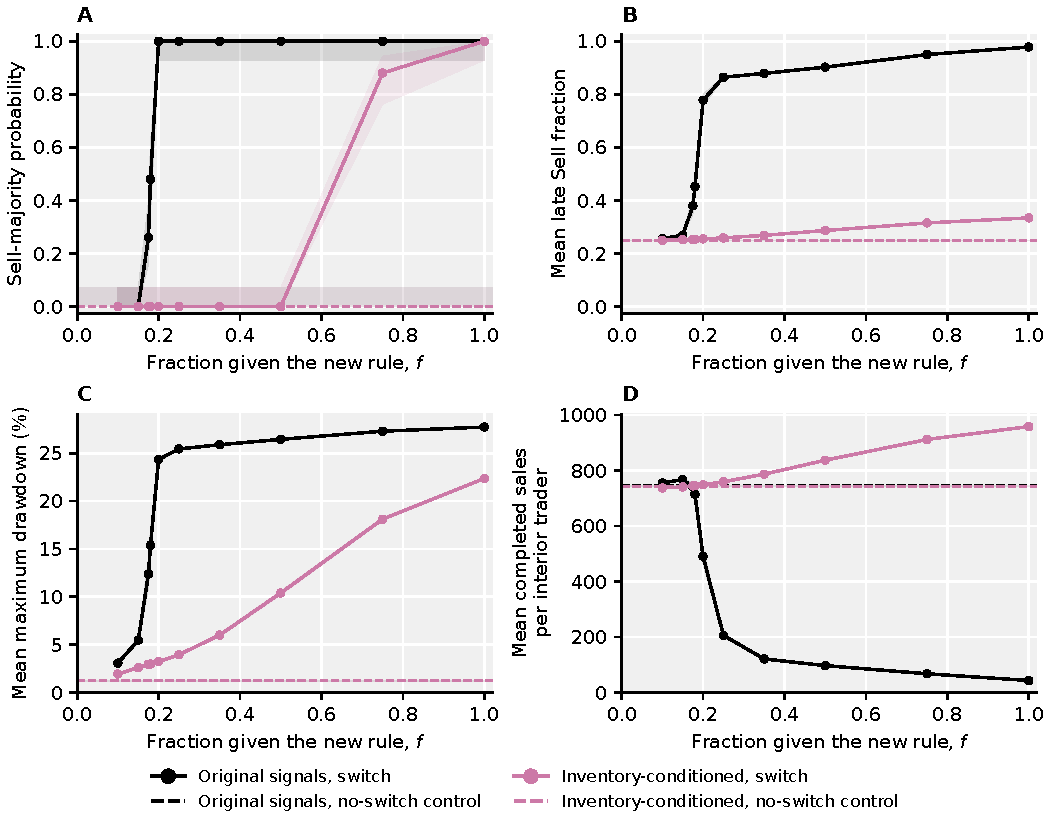
\includegraphics[width=\linewidth]{figs/FigS2-InventoryVisibility.pdf}
\caption{Inventory information in the primary setting: technical traders
held, dealer depth $h=100$, and grid size $L=64$. Black denotes original
signals and purple inventory-conditioned signals. Solid lines and points
denote switched markets; dashed horizontal lines denote the shared
no-switch controls. Each point used the same 50 starting markets and
3,000 post-intervention steps; joining lines guide the eye.
\textbf{(A)}~Probability of reaching a raw Sell majority, with Wilson
95\% intervals. \textbf{(B)}~Mean raw Sell fraction over the final 500
steps. \textbf{(C)}~Mean maximum quoted-price drawdown.
\textbf{(D)}~Mean completed sales per interior trader.
Bands in B--D are pointwise percentile 95\% intervals from 10,000
bootstrap samples of whole starting markets. The original sweep covered
fractions $f=0.10$ to 0.25; larger fractions were added under the
prespecified extension rule (Appendix~\ref{app:visibility}). Controls
retain Rule~19280 in both observation modes, so the change in control
outcomes measures the information intervention alone. The comparison
tests one hypothetical response to observing inventory.}
\label{fig:visibility}
\end{minipage}
\end{center}
